\section{Our Calling Convention}
We'll now talk more about the calling conventions we aim to use for our compiler, along with functions in general. Recall, from the previous section, that a \code{snek} program is defined by 
\begin{verbatim}
    <prog> := <defn>* <expr>

    <defn> := (fun (<name> <name>) <expr>)
        | (fun (<name> <name> <name>) <expr>)

    <expr> := ... 
        | (<name> <expr>) 
        | (<name> <expr> <expr>)\end{verbatim}
where \code{<defn>} means that our function declarations can either take one argument, or two arguments, respectively.

\subsection{Caller-Managed Stack Pointer}
An approach for calling functions is to have the caller (i.e., the function that is \emph{calling} a function) manage the stack pointer, \code{rsp}.

\subsubsection{Compiling the Definition}
Let's consider the following Rust code: 
\begin{verbatim}
    fn compile_definition(d: &Definition, labels: &mut i32) -> String {
        match d {
            Fun1(name, arg, body) => {
                ...
            }
            Fun2(name, arg1, arg2, body) => {
                let body_env = hashmap! {
                    arg1.to_string() => -1,
                    arg2.to_string() => -2
                };
                let body_is = compile_expr(body, 2, &body_env, 
                    &String::from(""), labels);
                format!(
                    "{name}:
                    {body_is}
                    ret"
                )
            }
        }
    }\end{verbatim}
This function is designed to compile a function declaration, specifically a function with one and two arguments. Some things to think about: 
\begin{itemize}
    \item Compiling a function is straightforward with this calling convention. All there is to the actual function is 
    \begin{itemize}
        \item The label (perhaps, the name of the function).
        \item The body of the function. 
        \item And then, \code{ret} for returning.
    \end{itemize}
    \item Note that the \emph{environment} is set up so that negative stack indexes are used. This way, the compiler ends up accessing \code{[rsp + X]}, i.e., accessing memory downwards as opposed to upwards. 
    \item In this approach, all the work of manipulating \code{rsp} is done by the \textbf{caller}.
\end{itemize}

\subsubsection{Compiling the Function Calls}
Now, let's look at the code that's responsible for compiling \emph{function calls}.
\begin{verbatim}
    fn compile_expr(
        e: &Expr,
        si: i32,
        env: &HashMap<String, i32>,
        brake: &String,
        l: &mut i32,
    ) -> String {
        match e {
            ...
            Expr::Call2(name, arg1, arg2) => {
                let arg1_is = compile_expr(arg1, si, env, brake, l);
                let arg2_is = compile_expr(arg2, si + 1, env, brake, l);
                let curr_word = si * 8;
                let offset = (si * 8) + (2 * 8);
                // With this setup, the current word will be at [rsp+16], 
                // which is where arg1 is stored. We then want to get rdi
                // at [rsp+16], arg2 at [rsp+8], and arg1 at [rsp], then call
                format!(
                    "
                    {arg1_is}
                    mov [rsp-{curr_word}], rax
                    {arg2_is}
                    sub rsp, {offset}
                    mov rbx, [rsp+16]
                    mov [rsp], rbx
                    mov [rsp+8], rax
                    mov [rsp+16], rdi
                    call {name}
                    mov rdi, [rsp+16]
                    add rsp, {offset}
                "
                )
            }
        }
    }\end{verbatim}
There are some things we need to make sure: 
\begin{itemize}
    \item We need to make sure we set \code{rsp} high enough so that it doesn't interfere with any of the temporary variables. 
    \item We also need to make sure we store the variables (arguments) in the right place before we actually call the function. \code{offset} is defined so that it will be used to move \code{rsp} above where we are, and then subtracting some more words, so we can make room for \code{rdi} and \textbf{two} arguments. 
    \item Note that, even though we have three items (\code{rdi} and the two arguments), we only need to move the stack index up by an additional 16 spaces, hence why we're adding \code{2 * 8}. % TODO why?
\end{itemize}


\subsubsection{Memory Layout}
With the above code for function \emph{calling}, let's look at a memory diagram of what's going on prior to calling a function. We know that \code{curr\_word} is defined as \code{si * 8}.
\begin{center}
    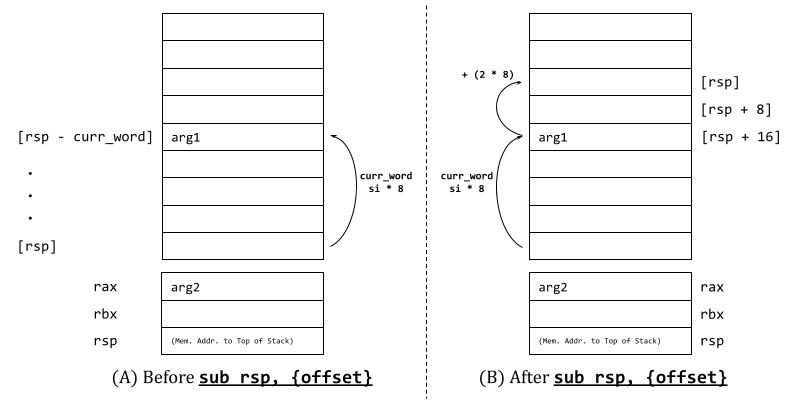
\includegraphics[scale=0.5]{assets/function_stack_mem.png}
\end{center}

So, what's going on? 
\begin{itemize}
    \item Before we call \verb|sub rsp, {offset}|, i.e., in diagram (A), 
    \begin{itemize}
        \item \code{[rsp]} is pointing to some initial return pointer (e.g., at a main expression or some function).
        \item \code{[rsp - curr\_word]} is where we stored \code{arg1} in the stack. Equivalently, \code{arg1} is stored \code{curr\_word} space ``above'' \code{rsp}.
        \item Remember that the result of \code{arg2} is stored in \code{rax}, since that was the last expression that was compiled.
    \end{itemize}

    \item After we call \verb|sub rsp, {offset}|, i.e., in diagram (B), 
    \begin{itemize}
        \item We moved \code{[rsp]} up by \code{(si * 8) + (2 * 8)} spaces, as seen by the two ``jumps'' in the diagram. 
    \end{itemize}
\end{itemize}
Our goal is to put \code{rdi} into \code{[rsp + 16]}, \code{arg2} into \code{[rsp + 8]}, and \code{arg1} into \code{[rsp]}. To make this happen, we need to move a few things around. That's where the following four assembly instructions, 
\begin{verbatim}
    mov rbx, [rsp+16]
    mov [rsp], rbx
    mov [rsp+8], rax
    mov [rsp+16], rdi\end{verbatim}
come from. To see how this works, let's visualize each line. 

\begin{center}
    \begin{tabular}{p{3in}|p{3in}}
        \textbf{After Running} & \textbf{Diagram} \\ 
        \hline 
        (Initial) & 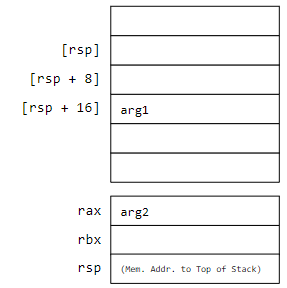
\includegraphics[scale=0.72]{assets/mem1.png} \\ 
        \hline 
        \code{mov rbx, [rsp + 16]} & 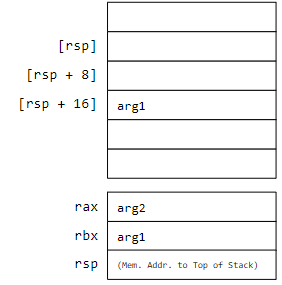
\includegraphics[scale=0.72]{assets/mem2.png} \\ 
        \hline 
        \code{mov [rsp], rbx} & 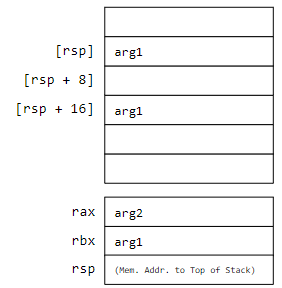
\includegraphics[scale=0.72]{assets/mem3.png} \\ 
        \hline 
        \code{mov [rsp+8], rax} & 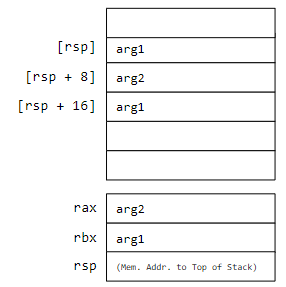
\includegraphics[scale=0.72]{assets/mem4.png} \\ 
        \hline 
        \code{mov, [rsp+16], rdi} &  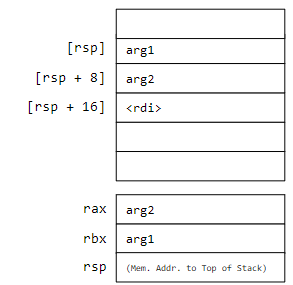
\includegraphics[scale=0.72]{assets/mem5.png} \\ 
    \end{tabular}
\end{center}

\textbf{Remarks:} 
\begin{itemize}
    \item Remember that the above only works for 2 arguments. For arbitrary arguments, the same idea still holds, but you need to generalize it.
    \begin{mdframed}
        \underline{Recall:} \emph{Before} we executed \code{sub rsp, ...}, we can imagine that \code{arg1} is at \code{[rsp - si * 8]}, \code{arg2} is at \code{[rsp - si * 8 - 8]}, \code{arg3} is at \code{[rsp - si * 8 - 16]}, and so on until \code{argN-1} is at \code{[rsp - si * 8 - 8(N - 1)]}. As usual, \code{rax} will hold \code{argN}.
    \end{mdframed}
    After we move \code{[rsp]}, we can expect \code{argN-1} to be at \code{[rsp + 16]}, \code{argN-2} to be at \code{[rsp + 24]}, and so on, with \code{arg1} being at \code{[rsp + 8(N + 1)]}. As usual, \code{rax} holds \code{argN}.
    
    \item \code{rdi} is a caller-saved register, hence why we're purposely saving it. 
    \item In this calling convention, as one might have guessed, we're putting everything on the stack. 
    \item While function arguments need positive offsets from \code{rsp}, \textbf{local variables} (temporaries) still use negative offsets from \code{rsp}. 
\end{itemize}
Now, after we do the \code{call} instruction, the memory diagram looks like 
\begin{center}
    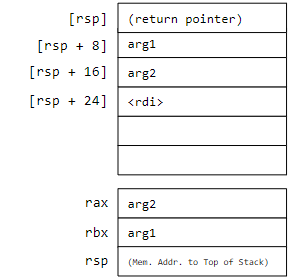
\includegraphics[scale=0.9]{assets/mem6.png}
\end{center}
In other words, the \code{call} instruction will move \code{rsp} up and write the return pointer into that word. At that point, it's clear that \code{arg1} and \code{arg2} are in the correct offsets.

\subsection{Callee-Managed Stack Pointer}
Suppose, instead, we want to have the function itself manage the stack pointer by moving it sufficiently enough. Then, at the start of a function call, suppose the memory diagram looks like this: 
\begin{center}
    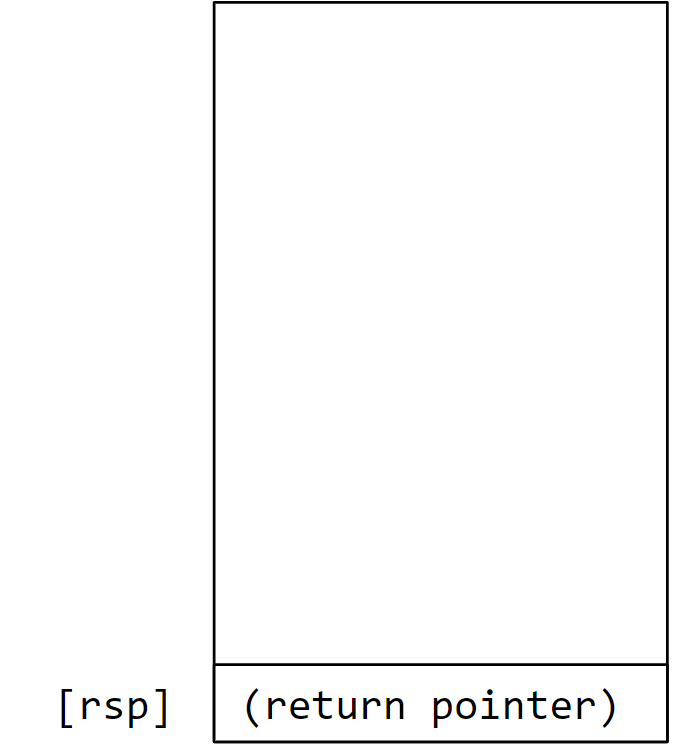
\includegraphics[scale=0.3]{assets/callee_stack_mnged_init.png}
\end{center}
Under this assumption where the callee manages the stack pointer, the first thing the function will do is \code{sub rsp} so that there's enough space for all local variables. That is, we should move \code{[rsp]} so that we end up with a memory diagram that looks like 
\begin{center}
    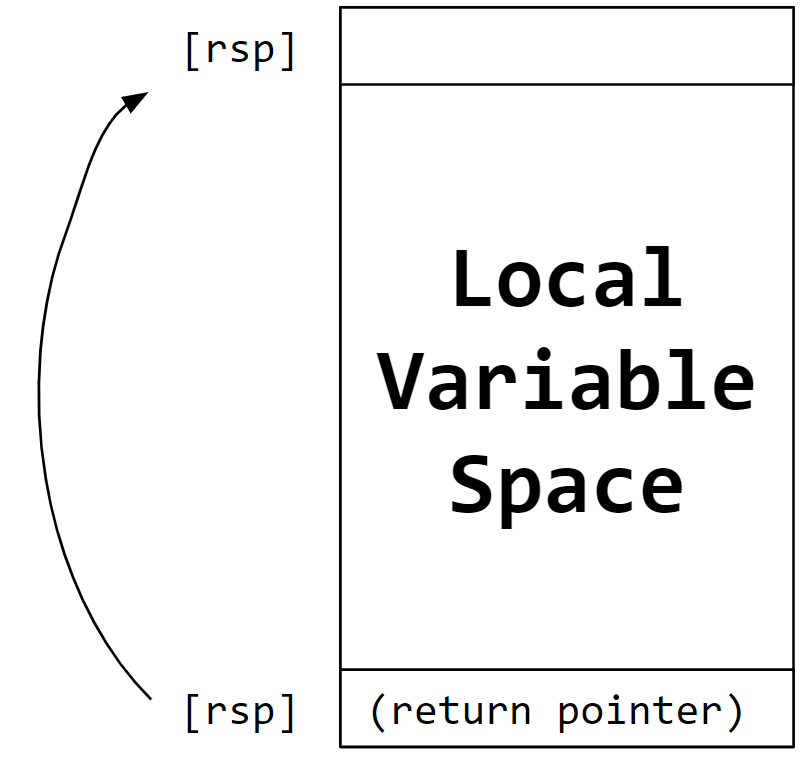
\includegraphics[scale=0.3]{assets/callee_stack_mnged.png}
\end{center}
Then, all lookups, including for argument and local variables, will have its location in the stack be positive offsets from \code{rsp}. There are some advantages to doing this, especially in relation to garbage collection.

\subsubsection{The Depth Function}
First, we need to know how many local variables are needed in the body of a function so we know how much we need to move \code{rsp} by. We can use the \code{depth} function to calculate the maximum stack index needed in an expression to store all local variables and temporaries. 

\bigskip 

Using the power of ChatGPT, along with some corrections, we have the following implementation:
\begin{verbatim}
fn depth(e: &Expr) -> i32 {
    match e {
        Expr::Num(_) => 0,
        Expr::True => 0,
        Expr::False => 0,
        Expr::Add1(expr) => depth(expr),
        Expr::Plus(expr1, expr2) => depth(expr1).max(depth(expr2) + 1),
        Expr::Let(_, expr1, expr2) => depth(expr1).max(depth(expr2) + 1),
        Expr::Id(_) => 0,
        Expr::Eq(expr1, expr2) => depth(expr1).max(depth(expr2) + 1),
        Expr::If(expr1, expr2, expr3) => {
            depth(expr1).max(depth(expr2)).max(depth(expr3))
        },
        Expr::Loop(expr) => depth(expr),
        Expr::Block(exprs) => exprs.iter().map(|expr| depth(expr)).max().unwrap_or(0),
        Expr::Break(expr) => depth(expr),
        Expr::Print(expr) => depth(expr),
        Expr::Set(_, expr) => depth(expr),
        Expr::Call1(_, expr) => depth(expr),
        Expr::Call2(_, expr1, expr2) => depth(expr1).max(depth(expr2) + 1),
    }
}\end{verbatim}

\subsubsection{Compiling the Definition}
With this in mind, we have 
\begin{verbatim}
    fn compile_definition(d: &Definition, labels: &mut i32) -> String {
        match d {
            Fun1(name, arg, body) => {
                ...
            }
            Fun2(name, arg1, arg2, body) => {
                let depth = depth(body);
                let offset = depth * 8;
                let body_env = hashmap! {
                    arg1.to_string() => depth + 1,
                    arg2.to_string() => depth + 2
                };
                let body_is = compile_expr(body, 0, &body_env, 
                    &String::from(""), labels);
                format!(
                    "{name}:
                    sub rsp, {offset}
                    {body_is}
                    add rsp, {offset}
                    ret"
                )
            }
        }
    }\end{verbatim}
We also need to do the same thing with the main expression (the main program):
\begin{verbatim}
    sub rsp, {offset}
    {main}
    add rsp, {offset}\end{verbatim}
where \code{offset} is defined by: 
\begin{verbatim}
    let depth = depth(&p.main); // p.main -> main program
    let offset = depth * 8;\end{verbatim}

\subsubsection{Changing Offsets in Code}
Recall how, before this section, any offsets we used were negative offsets (e.g., \verb|mov [rsp - {offset}], rax|). With this change, we now can use \textbf{positive offsets} (e.g., \verb|mov [rsp + {offset}], rax|). This scheme is similar to what most compilers like Rust, \code{g++}, and so on use. 